\documentclass{article}
\usepackage[%
    left=0.5in,%
    right=0.5in,%
    top=0.5in,%
    bottom=0.5in,%
]{geometry}%
\usepackage{minitoc}
\usepackage{mathtools}
\usepackage{multicol}
\usepackage{graphicx}
\usepackage{amssymb}
\usepackage{fixltx2e}
\usepackage{listings}
\usepackage{color}
\usepackage{hyperref}
    \hypersetup{ colorlinks = true, linkcolor = blue }
\usepackage{blindtext}
\definecolor{lightgray}{gray}{0.9}
\graphicspath{ {./} }
\usepackage{stmaryrd}


\newcommand\Hoaretriple[3]{%
  \llparenthesis\,#1\,\rrparenthesis
  \mathrel{#2}\nolinebreak 
  \llparenthesis\,#3\,\rrparenthesis
}

\newcommand{\inlinecode}[2]{\colorbox{lightgray}{\lstinline
[language=#1]$#2$}}
\newcommand{\worddef}[1]{\hyperref[sec:reference]{\textit{#1}}}

\begin{document}

\section{Hoare triples}
\begin{flushleft}
Triple assertion, usually writen as: \[ \Hoaretriple{\phi}{ P }{\psi} \]\\
Which (roughly) means: \\
If the program P is run in a stat that satisfies $\phi$, then the state resulting from P's execution will satisfy $\psi$.\\
\smallskip
$\phi$ - Is called \textit{precondition} of P and $\psi$ is called \textit{postcondition}
\end{flushleft}

\begin{flushleft}
Often, we do not want to put any constraints on the initial state; we
simply wish to say that, no matter what state we start the program in, the
resulting state should satisfy $\psi$. In that case the precondition can be set to $\top$.
\[ \Hoaretriple{\top}{ P }{\psi} \]\\
\end{flushleft}

\begin{flushleft}
We need a way of remembering the initial value of x, to cope with the fact
that it is modified by the program. Logical variables achieve just that: in the
specification
\[ \Hoaretriple{x=x_{0} \land x \geq 0}{ Fac2 }{y=x_{0}!} \]\\
The $x_{0}$ is a logical variable and
we read it as being universally quantified in the precondition. Therefore, this
specification reads: for all integers $x_{0}$, if \textit{x} equals $x_{0}$, $x \geq 0$ and we run the
program such that it terminates, then the resulting state will satisfy y equals $x_{0}!$.
\end{flushleft}

\section{Proof rules}
\begin{center}
  \makebox[\textwidth]{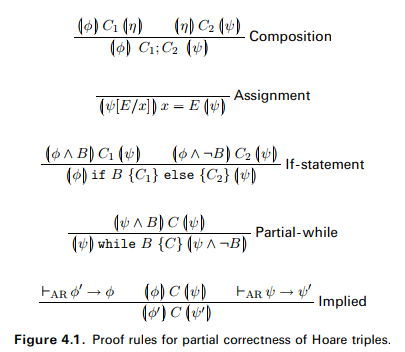
\includegraphics[scale=0.5]{Selection_021.png}}
\end{center}

\subsection{Composition}
\begin{flushleft}
\textit{Composition} given specifications for the program fragments $C_{1}$ and $C_{2}$ say
\[ \Hoaretriple{\phi}{ C_{1} }{\eta} \: \text{and} \: \Hoaretriple{\eta}{ C_{1} }{\psi} \]\\
where the postcondition of $C_{1}$ is also precondition of $C_{2}$, the proof rule allows us to derive a specification for $C_{1}\text{;}C_{2}$
\[\Hoaretriple{\phi}{ C_{1}\text{;}C_{2} }{\psi} \]\\
\end{flushleft}

\subsection{Assignment}
\begin{flushleft}
\textit{Assignment} rule has no premises and so is an axiom of logic. It states that we want to show that $\psi$ holds in the state following the assignment
$x = E$, we must show that $\psi[ \, E/x ] \,$ holds before the assignment.\\
We obtain $\psi[ \, E/x ] \,$  by taking $\psi$ and replacing all (free) occurences of $x$ in $\psi$ with $E$
\end{flushleft}

\subsection{If then else}
\begin{flushleft}
\textit{If then else} proof rule allows us to prove a triple by decomposing it into two triples on in which $B$ evaluates to true, and one where B evaluates to false.
\end{flushleft}

\pagebreak
\subsection{While}
\begin{flushleft}
The key idea of While rule is the \textit{invariant} $\psi$. In general, the body of the loop $C$ changes the values of the variables. The \textit{invariant} expresses a relationship between the values of these variables that is preserved by executing $C$.\\
It states that (provided B is true) if $\psi$ is true before $C$ is executed, and $C$ terminates, then $\psi$ will be true in the resulting state.
\end{flushleft}

\subsection{Implied}
\begin{flushleft}
If we have proved $\Hoaretriple{\phi}{ C }{\psi}$ and we have formula $\phi \text{'}$, which implies $\phi$ and another formula $\psi$, which implies $\psi \text{'}$. Then we can also prove that 
\[ \Hoaretriple{\phi \text{'}}{ C }{\psi \text{'}} \]
\end{flushleft}

\pagebreak
\section*{Reference section} \label{sec:reference}
\begin{description}
	\item[placeholder] \hfill \\ placeholder
\end{description}
\end{document}
